%
% Modified by Megan Patnott
% Last Change: Jan 18, 2013
%
%%%%%%%%%%%%%%%%%%%%%%%%%%%%%%%%%%%%%%%%%%%%%%%%%%%%%%%%%%%%%%%%%%%%%%%%
%
% Modified by Sameer Vijay
% Last Change: Tue Jul 26 2005 13:00 CEST
%
%%%%%%%%%%%%%%%%%%%%%%%%%%%%%%%%%%%%%%%%%%%%%%%%%%%%%%%%%%%%%%%%%%%%%%%%
%
% Sample Notre Dame Thesis/Dissertation
% Using Donald Peterson's ndthesis classfile
%
% Written by Jeff Squyres and Don Peterson
%
% Provided by the Information Technology Committee of
%   the Graduate Student Union
%   http://www.gsu.nd.edu/
%
% Nothing in this document is serious except the format.  :-)
%
% If you have any suggestions, comments, questions, please send e-mail
% to: ndthesis@gsu.nd.edu
%
%%%%%%%%%%%%%%%%%%%%%%%%%%%%%%%%%%%%%%%%%%%%%%%%%%%%%%%%%%%%%%%%%%%%%%%%
%
% Chapter 1
%

%\documentclass{article}
%\usepackage{mathtools}

\chapter{INTRODUCTION}

In computer simulation of condensed phase molecular systems, molecules are commonly represented by atomic sites that interact by a parametrized forcefield. This forcefield aims to reproduce observable phenomena, by incorporating the proper physics into the simulation. There are mainly two types of interaction; intramolecular and intermolecular, which determines the static and dynamic properties of the molecular systems. Intramolecular interaction is the interaction within a single molecules which includes, bonding, bending, torsion etc whereas intermolecular interaction is the interaction between two or more molecules which includes van der Waals and electrostatic interactions due to full or partial charges located on or near the atomic sites. The computation of these electrostatic interactions is the most expensive portion of a molecular simulations. Due to this, there have been significant efforts to develop practical, efficient, and accurate methods for evaluating electrostatic interactions. 

The Ewald method is one of the most well known and accurate method but it is computationally expensive scaling as O($N^2$), where $N$ is the total number of particles. The appropriate selection of damping paramenter and suitable algorithm can decrease computational cost to O($N^{3/2}$)\cite{Perram88}. Modification of the Ewald method, including a particle mesh and fast Fourier transform (FFT) have decreased its cost down to O($N\log N$) \cite{Shimada93, Luty95, Darden93,Essmann95}. But these modified Ewald methods (particle mesh Ewald (PME), particle-particle particle-mesh Ewald (P3ME)) are still computationally expensive. In addition to this, the Ewald method requires an inherent periodicity which can be problematic in a number of protein/solvent and ionic solution environments \cite{Roberts94,Roberts95,Luty96,Hunenberger99a,Hunenberger99b,Weber00,Gezelter06}. To address these problems a lot of interest is currently growing in developing efficient real space electrostatic methods which scales linearly with the system size i.e. O($N$). This method was originally proposed by wolf \textit{et al.} \cite{Wolf99} and extended initially by Zahn \textit{et al.}\cite{Zahn02} then by C.J. Fennell and J. D. Gezelter \cite{Gezelter06}. All these methods were limited to charge-charge interactions between atomic cites. Our research developed real-space electrostatic interaction methods for higher order charge-multipoles (dipoles and quadrupoles) and studied their applications and performance in various condensed phase environments. This research also studied various static, dynamic, and dielectric properties for molecular systems using newly developed real space methods. 

%which the conditionally convergent sum of the electrostatic energy is converted into two absolutely convergent terms, one being evaluated in real space and the other in reciprocal space \cite{ Allen87, deLeeuw80, Ewald21,Smith81}. Calculation of the reciprocal term is very inefficient which makes
%
%Often this includes a Lennard-Jones potential and electrostatic interactions due to full or partial charges located on or near the atomic sites. 

This dissertation consists of five chapters. First chapter is an introductory chapter initially outlines the background and motivation of the research. It also briefly  discusses the basic principles of widely used molecular simulation methods: Molecular Dynamics (MD) and Monte Carlo (MC) simulations, where the newly developed electrostatic methods are very useful. Similarly this chapter also describes traditional Ewald as well as various improved Ewald based methods: P3ME, PME, and Multiple-based Ewald. Additionally it presents the problems caused due to the spherical truncation in real-space methods and discusses various technique implemented to resolve this problem in the past.

Chapter 2 presents the mathematical formulation of our newly developed real-space electrostatic methods: Gradient-shifted Force (GSF), Shifted-potential (SP), and Taylor-shifted force (TSF). It also compares energy constant evaluated  using newly developed methods with analytical results for different types dipolar and quadrupolar crystals.

The accuracy newly developed methods have been tested against Ewald in Chapter 3. Furthermore various static and dynamic properties evaluated from real space methods are also compared with traditional Ewald method. The test of total energy conservation is very important in MD simulations which is also studied in this chapter. 

Chapter 4 describes three different ways of evaluating the dielectric properties for dipolar and quadrupolar liquids using Flcutuation, Perturbation, and Potential of Mean Force (PMF) methods. This chapter also explores the correction factor required to obtain correct dielectric using  GSF, SP, and TSF methods. In addition, the dielectric properties; susceptiblity and dielectric constant, obtained using all three different methods are compared with each other as well as with previous simulation result in case of Stockmayer fluid.

Finally Chapter 5 summarizes, draw conclusion and discusses future directions, applications, and limitations of my research. 

\section{Molecular Dynamics (MD) Simulation}

Molecular dynamics is computer simulation method for studying static and dynamic properties for molecular systems. In this method, each atom or molecule interacts with other molecules in the system and evolve dynamically following classical equation of motion. The numerical step-by-step process for MD is outlined in Figure \ref{fig:MD}. 
    
\begin{figure}[tpb]
  \begin{center}
    \centerline{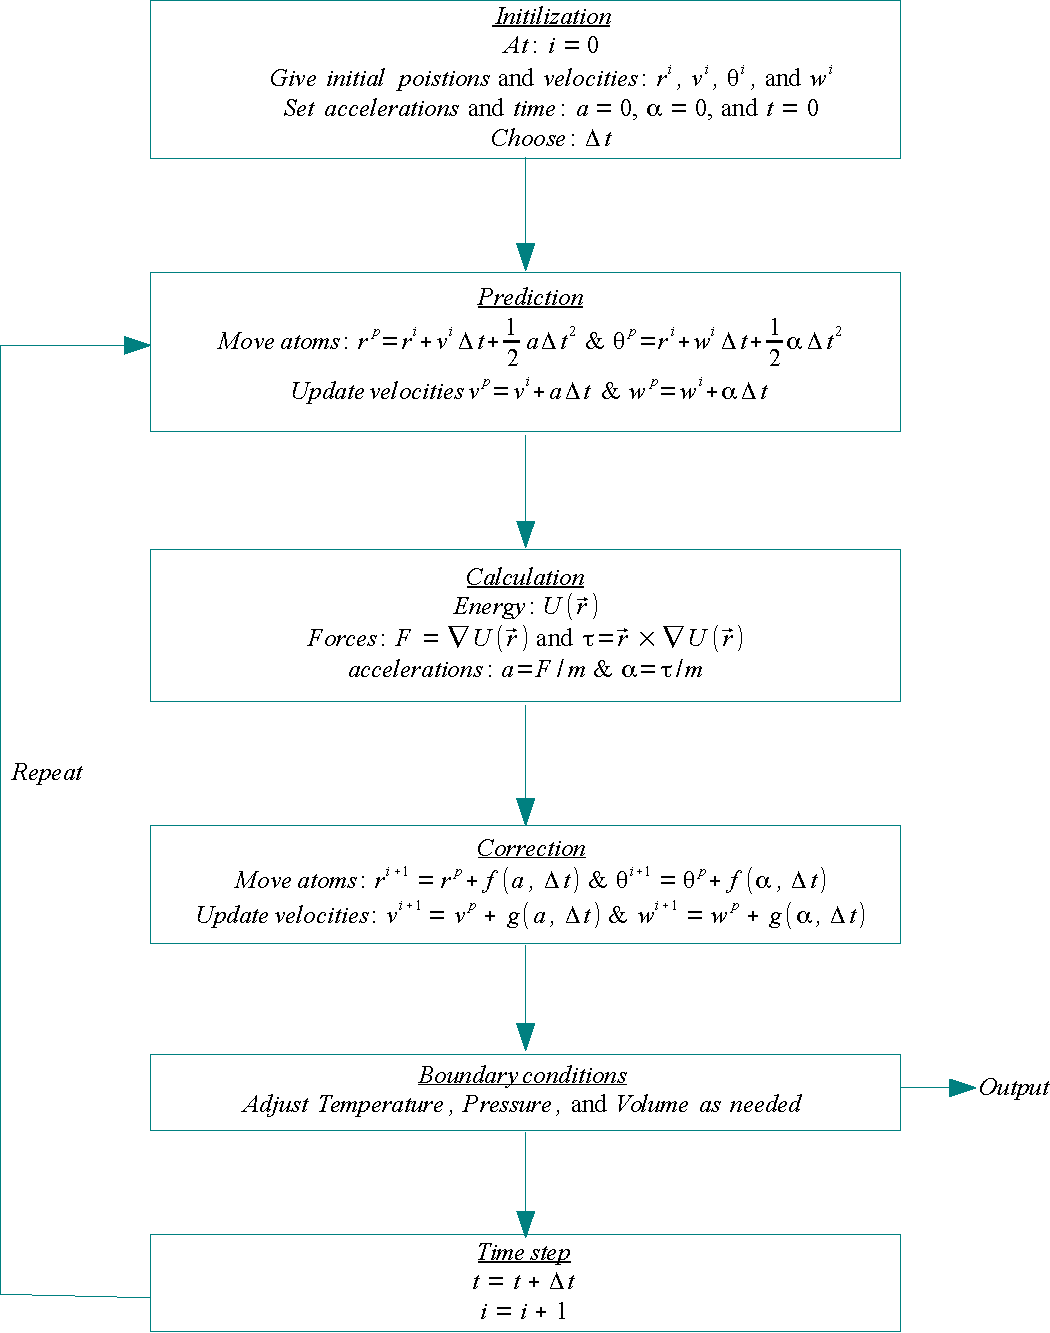
\includegraphics[scale=0.8]{MD_flowchart.pdf}}
    \caption{Schematic figure showing step-by-step process in Molecular dynamics simulation algorithm.}
    \label{fig:MD}
  \end{center}
\end{figure}

In MD simulation, first of all molecules are initialized by assigning their initial positions and velocities at given boundary conditions. Molecules are usually initialized in such a way so that system does not take very long time to reach equilibrium. Before moving a molecule in the system, we need to evaluate its potential energy which is mainly due to intramolecular interactions within the molecule itself as well as intermolecular interactions with all other molecules in the system. We can write the potential energy for a molecule in a system as shown in below:
\begin{equation}
U(\mathbf r) = \overbrace{U_{bond} + U_{bend} + U_{torsion}}^{Intramolecular\; interactions} + \overbrace{U_{electrostatic} + U_{van\;der \;Waals}}^{Intermolecular\;interactions} + ...
\label{eq:potential}
\end{equation}   
In equation \ref{eq:potential} the energy due to bonding, bending, and torsion represents intramolecular interactions whereas electrostatic and van der Waals represents intermolecular interactions. The force and torque acting on the molecule is obtained using following equations.

\begin{subequations}
\begin{gather}
\mathbf F (\mathbf r) = \nabla_r U(\mathbf r) \\
\mathbf {\mathbf{T}}(\mathbf r) = \mathbf r \times \nabla_r U(\mathbf r).
\end{gather}
\label{eq:forceTorque}
\end{subequations}

The force and torque provides the required dynamics to the molecule at a given time step. The same process is repeated for every molecules in the system. Once the molecules move forward by time step following prescribed equation of motion, their positions and velocities are adjusted according to applied boundary conditions (i.e temperature, pressure, volume etc) in the system. After adjusting positions and velocities, again we can evaluate the potential energy for each molecule and repeat same process till the simulation completes its predetermined simulation time.
 
In MD simulations, the intermolecular interactions are most expensive parts of simulation. Among them van der Waals interaction is short range interaction usually described by Lennard-Jones (LJ) potential can be written as,

\begin{equation}
U_{LJ}(r) = 4\epsilon \left[\left(\frac{\sigma}{r} \right)^{12} - \left(\frac{\sigma}{r} \right)^6\right],
\label{eq:LJ}
\end{equation}
where $\sigma$ is diameter of a molecule and $\epsilon$ determines well depth of the attractive potential. Above equation \ref{eq:LJ} clearly shows it decays much faster with the distance therefore considered as short-range interaction. The repulsive part of the  LJ potential $ \textit{~}\frac{1}{r^{12}}$ prevents two or more molecules to occupy same position. The electrostatic interactions are considered as long-range interaction. If we consider charge-charge interactions between molecules then they interact with Coulomb's law 

\begin{equation}
U_{electrostatic}(r) = \frac{1}{4\pi \epsilon_o}\frac{q_1 q_2}{r}.
\label{eq:Coulomb}
\end{equation}
Equation \ref{eq:Coulomb} shows that electrostatic interaction decay much slower with the distance i.e. $ \frac{1}{r}$. If we consider lowest order moment in the molecule as a dipole then the electrostatic interaction falls off by $\frac{1}{r^3}$. Even for considering lowest order moment in molecule as quadrupole, the electrostatic interaction decays as $\frac{1}{r^5}$ which is slower than LJ interaction. Since the electrostatic interaction decays slowly we need to consider large number of molecules around a molecule to capture right physical behaviour due to interactions. But it causes computational inefficiency when considered interactions with large number of molecules around it. The most important challenge in the molecular dynamics communities have been to capture right electrostatic behaviour of a molecule considering small number molecules around it. There have been many efforts in the past to develop efficient and accurate algorithms to evaluate electrostatic interaction in molecular simulation, which will be discussed in detail in the following section \ref{sec:ElectMethod} . Still those electrostatic methods have got some limitations. In addition to that those methods can also be generalized to higher order charge-multipoles. We will also discuss about how our newly developed electrostatic methods will resolve these issues.    

%The main purpose of our research is developing accurate and efficient electrostatic interaction methods considering small number of molecules around a given molecules.  
Real liquid systems consists of very large number of molecules. But for computational efficiency only small number of particles (few thousands) are usually considered in molecular simulations. On the other hand, if we want to study and predict bulk properties of the material considering small number of molecules, the large fraction of molecules will be near the edge of the sample contributing huge surface effect. To eliminate surface effect, Periodic Boundary Conditions (PBC) have long been employed in various simulations \cite{Born1912}.
 
\subsection{Peridic Boundary Condition (PBC)}
In PBC, the simulation box is replicated throughout the space to form an infinite lattice. In the course of simulation, if a molecule moves in the central box then its images in every replicated boxes also move in the similar fashion. Similarly if a molecule leaves the central box then the one of its images will enter the box through opposite face as shown in Figure~\ref{fig:PBC} to conserve total number of particle in a central box. Therefore the system acts like there is no wall at the boundary of the central box which eliminates the surface effect in the computation. In this method if we want to evaluate potential energy of a molecule, we can consider its interactions with nearest molecules or images using minimum image convention \cite{Allen04}. Even if you use minimum energy convention, for each molecule we need to calculate large number of pairwise distances at each simulation time step. Consider a system of N molecules, if we want to evaluate potential energy for a $i^{th}$ molecule we need to find its distances $r_{ij}$ with every $j^{th}$ molecules or images in the system. To evaluate total energy of the system, $\frac{1}{2} N (N-1)$ number of distinct distances should be calculated at each time step, which makes computation very expensive. If the interaction between molecules is short-ranged then we can consider small distance around the molecule and assume that molecule only interacts with the molecules within that region. Providing small cutoff region around the molecule and evaluating interactions only within that region, we can make MD simulation very efficient.  

  
\begin{figure}[tpb]
  \begin{center}
    \centerline{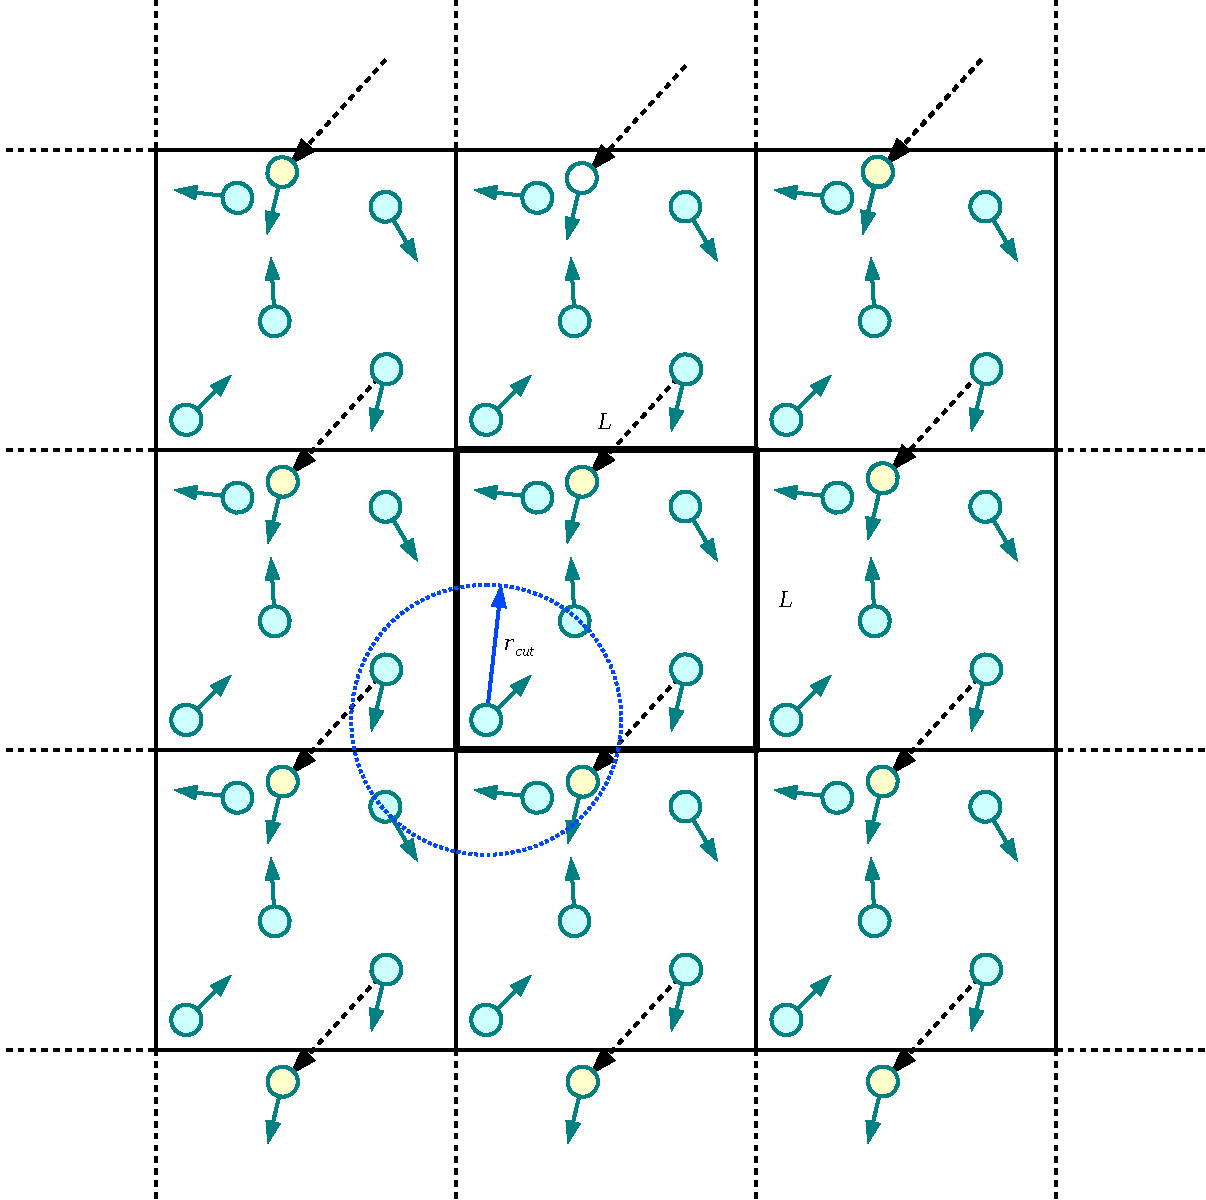
\includegraphics[scale=0.8]{PBC.pdf}}
    \caption{Periodic Boundary Condition for two dimensional (2D) molecular system. The central 	box is outlined using thicker line and replicated through out the plane to form 2D lattice. Usually in simulations, the potential energy of a molecule is evaluated considering interactions with the molecules and images within a cutoff region as shown in blue circle}
    \label{fig:PBC}
  \end{center}
\end{figure}

\subsection{Spherical truncation and Neighbour list }
Often in liquid simulations the small spherical cutoff region ($r_{cut}$) is considered around a molecule to take account of its interaction with molecules, beyond which there is no interaction between the molecules. Consider a system of molecules with box size $L$ employed in PBC then $r_{cut}$ should be less than $L/2$ in simulation. If $r_{cut} > L/2$ then molecule may interact with other molecules as well as their images at the same time which is problematic in molecular dynamic simulation. The spherical truncation implemented in PBC is shown in figure \ref{fig:PBC}. 

But evaluating every pair distances between molecules at every time step to determine whether or not a particular molecule is within cutoff region is computationally expensive. Therefore the cutoff sphere of $r_{cut}$ is surrounded by the another larger sphere of radius $r_{list}$ as shown in figure \ref{fig:neighbourList}. At the beginning of the simulation a list of the molecules i.e. neighbour list is constructed around each molecule for which the pair separation $r_{ij} < r_{list}$. For few time step, only the molecules in the neighbour list are selected to check whether or not they are within the cutoff sphere. After few time step, neighbour list is again reconstructed by evaluating pair distances between the molecules. This reconstruction time for the neighbour list is mainly determined by the dynamics of the molecules in the simulation.  
\begin{figure}[tpb]
  \begin{center}
    \centerline{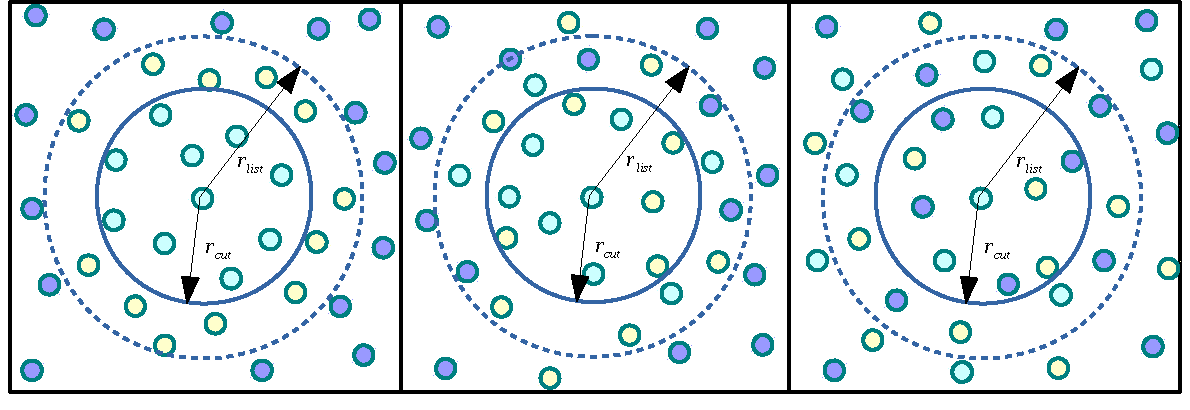
\includegraphics[scale=0.8]{neighbourList.pdf}}
    \caption{Region of neighbour list around the cutoff sphere. The molecules in cutoff region, neighbour list, and outer region are indicated by green, yellow, and violet circles. The neighbour list  should be reconstructed before molecules in the outer region starts to penetrate cutoff region.}
    \label{fig:neighbourList}
  \end{center}
\end{figure}


\section{Monte Carlo (MC) Simulation}
To study any physical and statistical properties of the system, we need to generate large number of different configurations with the consideration of constraints imposed in the system. Monte Carlo method uses probabilistic interpretation of the system to generate various configurations of the system. Each configuration depends only upon its processor but does not depend on the all the other configurations that were visited previously. For a canonical system, the probability of obtaining a given configuration is given by Boltzmann factor, $e^{-\frac{\Delta E}{k_B T}}$. Metropolis et. al developed the selection criteria for acceptance of the subsequent configuration of the system \cite{Metropolis53}. According to their method, the new configuration of the system is accepted either  $\Delta E < 0$ or  $e^{-\frac{\Delta E}{k_B T}} > r$, where $r$ is the random number between 0 and 1. The evaluation of the potential energy difference between subsequent configurations i.e $\Delta E$ is very important in the MC simulation. For computational efficiency, this method also utilize pairwise electrostatic interactions including cutoff region $r_{cut}$ as well as periodic boundary condition. Therefore developing efficient and accurate electrostatic interaction method has always been subject of interest in the MC communities. 

\section{Electrostatic Methods}
\label{sec:ElectMethod}
Consider a system of $N$ particles in a cubic box of length $L$  replicated infinitely in the 3D-space then the electrostatic potential energy of the particle with charge $q_i$ and located at $r_i$ is given by
\begin{equation}
U_i =  \sum_n^{'}{ \sum_{j=1}^N {\frac{q_i q_j}{\lvert {\mathbf{r}_i-\mathbf{r}_j + \mathbf{n}L}\rvert}}},
\label{eq:electrostatic}
\end{equation}
where $q_j$ represents all other charges located at position $\mathbf{r}_j$ or in periodic replicas. Similarly $\mathbf{n}$ is the cell-coordinate vector can be expressed as $\mathbf{n}L = n_1 L \;\hat{x} + n_2 L\;\hat{y} + n_3 L\;\hat{z}$, where $n_1,n_2, \text{and}\; n_3$ number of cell along $x$, $y$, and $z$ directions and can vary from 0 to \textit{infinity}. The prime in the first sum indicates that $i =j $ should be ignored for central box i.e. $n = 0$. The factor $\frac{1}{4\pi\epsilon_o}$ has been dropped in the equation \ref{eq:electrostatic} for simplicity. The total potential energy of the system can be evaluated as,
\begin{equation}
U = \sum_{\substack{i=1 \\ i\neq j}}^N{U_i} = \frac{1}{2}\sum_n^{'}{\sum_{i=1}^N { \sum_{j=1}^N {\frac{q_i q_j}{\lvert {\mathbf{r}_i-\mathbf{r}_j + \mathbf{n}L}\rvert}}}},
\label{eq:totalElectrostatic}
\end{equation}
where factor of $\frac{1}{2}$ in the second part of the equation is due to removing $i \neq j$ in the summation. Since the electrostatic interaction (Coulomb interactions) is the long-range interactions hence very time consuming in the molecular simulation. On the other hand the potential energy evaluated using equation \ref{eq:Electrostatic} converges conditionally to the correct value depending on the order of summation taken into account during  calculation\cite{Allen89}. Therefore there have been many efforts to reduce computational time and remove its conditional convergent behaviour during simulation will be discussed in the following subsections.  

\subsection{Ewald Method}
This method was originally proposed by \texit{Ewald} in 1921 to evaluate electrostatic interactions in PBC. In this method, the electrostatic interaction  can divided into two rapidly converging real and reciprocal space sums as well as a constant self-term \cite{Toukmaji96}.  
\begin{subequations}
\begin{gather}
U_{real} = \frac{1}{2} \sum_{i,j}^{N}{\sum_{n}^{'}{{q_i q_j}\frac{\mathrm{erfc}(\alpha r_{ij,n})}{r_{ij,n}}}}, \label{eq:ewald1}\\
U_{reciporcal} = \frac{1}{2\pi V}\sum_{i,j}^{N}{\sum_{\mathbf{m} \neq 0}\frac{\exp(-(\pi \mathbf{m}/\alpha)^2 + 2\pi i \mathbf{m}.\mathbf{r}_{ij})}{\mathbf{m}^2}},\label{eq:ewald2} \\
U_{self} = -\frac{\alpha}{\sqrt{\pi}} \sum_{i =1}^{N} {q_i}^2 ,\label{eq:ewald3}
\end{gather}
\end{subequations}
where $V$ is the volume of the simulation box and $\mathbf{m}$ is a reciprocal-space vector. The self-term in the equation \ref{eq:ewald3} is to remove artificial interactions of a charge with its images located in the periodic replicas of the box. Since  $\mathrm{erf}(x) + \mathrm{erfc}(x) = 1$ we can write \ref{eq:totalElectrostatic} as,
\begin{equation}
U = \frac{1}{2}\sum_n^{'}{\sum_{i=1}^N { \sum_{j=1}^N {q_i q_j}}}\frac{\mathrm{erfc}(\alpha r_{ij,n})+\mathrm{erf}(\alpha r_{ij,n})}{r_{ij,n}},
\label{eq:efforFuncElectrostatic}
\end{equation}
where $\alpha$ is damping parameter. The equation \ref{eq:ewald1} is obtained by taking complementary error function term and the equation \ref{eq:ewald2} can be obtained taking Fourier transform of the error function term in equation \ref{eq:efforFuncElectrostatic}.
 
Physically each point charge in the system can be assumed to be surrounded by a Gaussian distribution of equal magnitude and opposite signed charge (see figure \ref{fig:Ewaldsum}) with density,

\begin{equation}
\rho_i (r) = q_i \left(\frac{\alpha}{\sqrt{\pi}}\right)^3 \exp(-\alpha^2 r^2),
\label{eq:chargeDistribution}
\end{equation}
where $\alpha$ is a damping parameter determines the distribution of the charge, $r$ is the position from the center of distribution. The imposed charge distribution around a charge screens the interactions between the charges making interaction a short-ranged and converges rapidly with distance. The imposed Gaussian distribution is counteracted by another Gaussian distribution of the charge with same magnitude but opposite in sign. The sum of potential energy due to second type of charge distributions converge rapidly in the reciprocal space. 

\begin{figure}[tpb]
  \begin{center}
    \centerline{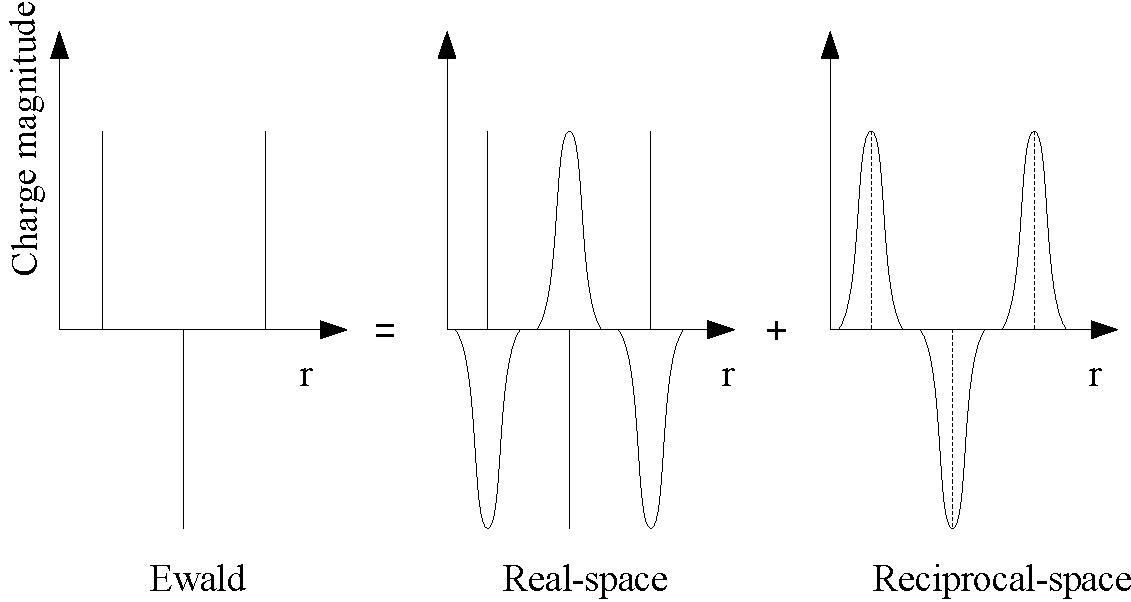
\includegraphics[scale=0.8]{Ewaldsum.pdf}}
    \caption{In Ewald method point charge is surrounded by the Gaussian distribution of the equal and opposite-signed charge evaluated in real-space. These Gaussian distributions are compensated by the corresponding opposite-singed distribution of the charges calculated in the reciprocal-space }
    \label{fig:Ewaldsum}
  \end{center}
\end{figure}

\subsection{Fourier-based Ewald Methods}

\subsection{Multipole-based Ewald Methods}

\subsection{Real Space Methods}


